% !TEX root = main.tex
\section{Introduction}
\label{sec:Introduction}
When designing any radio communication system, trade-offs has to be made between bandwidth, power, system complexity and bit rate. For a given bandwidth and transmit power, the bit rate could be varied by using different modulation schemes. As higher order modulation schemes require higher $\frac{E_b}{N_0}$, choosing optimum modulation scheme would require knowledge about the radio channel in order to maintain low enough BER at the receiver. This knowledge may be obtained by adding complexity in form of a feedback channel from receiver to transmitter. By performing some kind of error detection, the receiver may send information about detected error rates back to the transmitter. This enables the system to adapt the data rate to the state of the radio channel, and thus provide better QoS for given power and bandwidth. 

In this paper, we present a radio communication system with this kind of feedback structure. The system is to be seen as a "proof of concept" and the goal is not to propose a complete radio system for commercial use. As the main goal of the system is to demonstrate this feedback feature, all design choices are made with this in mind. We chose for instance not to implement any source encoding because it is not necessary to fulfil the purpose of our system, but would be highly favourable in a commercial system. 

The adaptable quality is obtained by implementing a feedback path from the receiver to the transmitter. Figure \ref{fig:block_toplevel} shows a top level block diagram of the proposed system. The figure shows that speech data is sent in the forward path from transmitter to receiver, and the number of detected errors is sent in the feedback path from receiver to transmitter. The forward and feedback paths will be referred to as the \textit{data path} and the \textit{BER path} respectively. 
% !TEX root = main.tex
\begin{figure}[htbp]
\centering
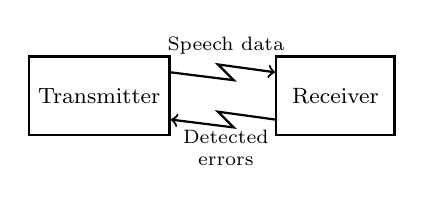
\begin{tikzpicture}[                
                    box/.style={
            		draw,
			thick,
            		text centered,
            		minimum width=1.5cm,
            		minimum height=1cm,
			font=\footnotesize,
			align=center,
			anchor=center,
            	} ]
	

\draw 
(0,0) node[box] (trans) {Transmitter}
(3,0) node[box] (rec) {Receiver}
(rec.west) ++(0,0.3) coordinate[](data_in) {}
(trans.east) ++(0,0.3) coordinate[](data_out) {}
(rec.west) ++(0,-0.3) coordinate[](ber_in) {}
(trans.east) ++(0,-0.3) coordinate[](ber_out) {}
;
\draw[thick, ->] (data_out) -- ++(0.8, -0.1) -- ++(-0.2, 0.2) node[above, align=center, font=\scriptsize, anchor=south, xshift=0.1cm]{Speech data} -- (data_in);
\draw[thick, <-] (ber_out) -- ++(0.8, -0.1) -- ++(-0.2, 0.2) node[below, align=center, font=\scriptsize, anchor=north, yshift=-0.1cm, xshift=0.1cm]{Detected \\ errors} -- (ber_in);

	
\end{tikzpicture}
\caption{Top level block diagram of proposed system. Speech data is sent in the forward path from transmitter to receiver and the number of detected errors is sent back from receiver to transmitter.}
\label{fig:block_toplevel}
\end{figure}

Throughout this paper, we will use the word \textit{transmitter} when referring to the radio module that is transmitting the speech data and \textit{receiver} when referring to the module that is receiving it. This is not to be confused with the terms TX and RX, which we use when referring to the transmit and receive port on each radio module. 

The system is implemented using the software defined radio USRP-2901\cite{USRP2901} from National Instruments, which contains all necessary RF hardware. All the software parts of the system is implementing in C++ and is executed on a standard personal computer. Pre-written C-libraries are used for the parts of the system concerning interface to the USRP, the computer sound card etc. These parts will not be explained in detail, but references to the libraries will be given. For the remaining parts of the system, we focus on explaining the implementation on a behavioural level and detailed descriptions of C code implementations is avoided. 

This paragraph will give tell the reader what to find in the remaining sections of the paper. 
